\chapter{Temperature-controlled experiment box}\label{ch:experiment_box}

Having an environment with a stable temperature is crucial for many optics experiments, as it reduces thermal expansion or contraction leading to drift in optical alignment as well strain changes in non-PM single mode optical fibers resulting in polarization state drift. For the network experiment, most of the optics for launching beams at the atoms are glued inside the vacuum chamber, but the external MOT beams and myriad of optical fibers are still susceptible to thermal drift. To mitigate this, both nodes live in a table-top enclosure with a temperature control loop. 

The enclosure or "experiment box" (Fig. \ref{fig:experiment_box_frame}) is constructed with a frame made from 1" x 0.5" 8020 bars and removeable panels made from 0.25" Alumalite plus a layer of microwave-damping foam (Laird ECCOSORB® QR-13AF) on the inner side of the panels held in place by flameless flame retardant paper (Pacon). The paper prevents degraded foam particles from dropping onto the optics while mitigating risk of a laser-induced fire. The panels also include sections with electrical feedthroughs including BNC, SMA, USB, XLR, and ethernet. The overall design of the box was based on the one described in \cite{kwon2019rydberg}, with some minor modifications from Arian Noori and Ethan Lu.

\begin{figure}[!ht]
    \centering
    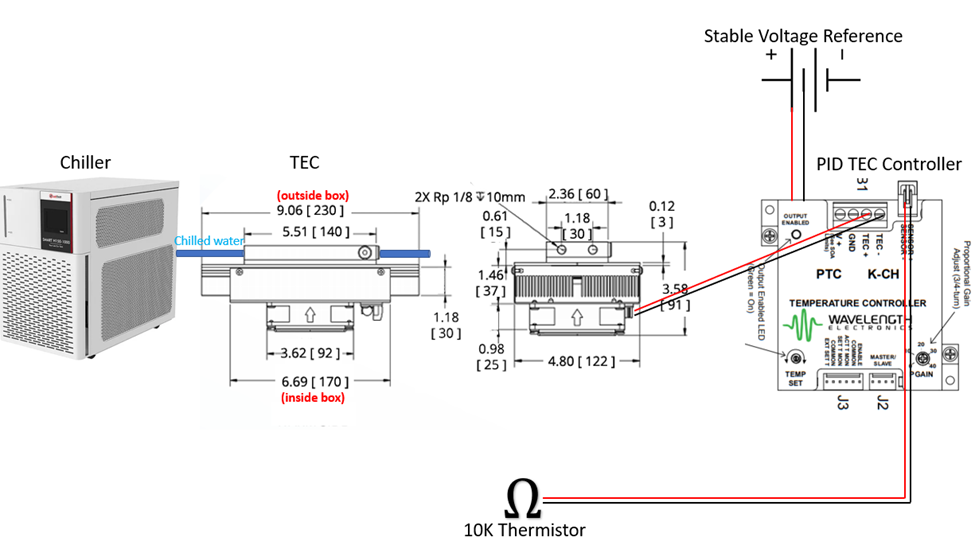
\includegraphics[width=1\textwidth]{Images/chiller_TEC_control_diagram.pdf}
    \caption{Chiller, TEC, and TEC controller connections. Courtesy Arian Noori.}
    \label{fig:box_TEC_control}
\end{figure}

A temperature control loop, shown schematically in Fig. \ref{fig:box_TEC_control} is used to keep the air inside the box stable within about 0.1 $^{\circ}$C (typical). Six thermoelectric cooler (TEC) units (Laird TEC LA-075-24-02) with fans are placed around the base of the box in order to exchange heat between the air in the box and chilled water. The water is chilled and pumped through the closed loop by a LabTech Smart H150-1000 water chiller. Heat flow mediated by the TECs is regulated by PI loops implemented with one Wavelength electronics PTC5K-CH TEC controller per TEC, where each controller reads the value of a 10k thermistor placed in the air near the TEC for that channel Fortuitously, the TEC controllers are analog, and therefore do not radiate magnetic noise from pulse-width modulation which can contribute to qubit decoherence. Some mechanical design details are shown in Figs. \ref{fig:box_TEC_mount_side} and \ref{fig:box_TEC_mount_back}.

\newpage

\begin{sidewaysfigure}[!ht]
    \centering
    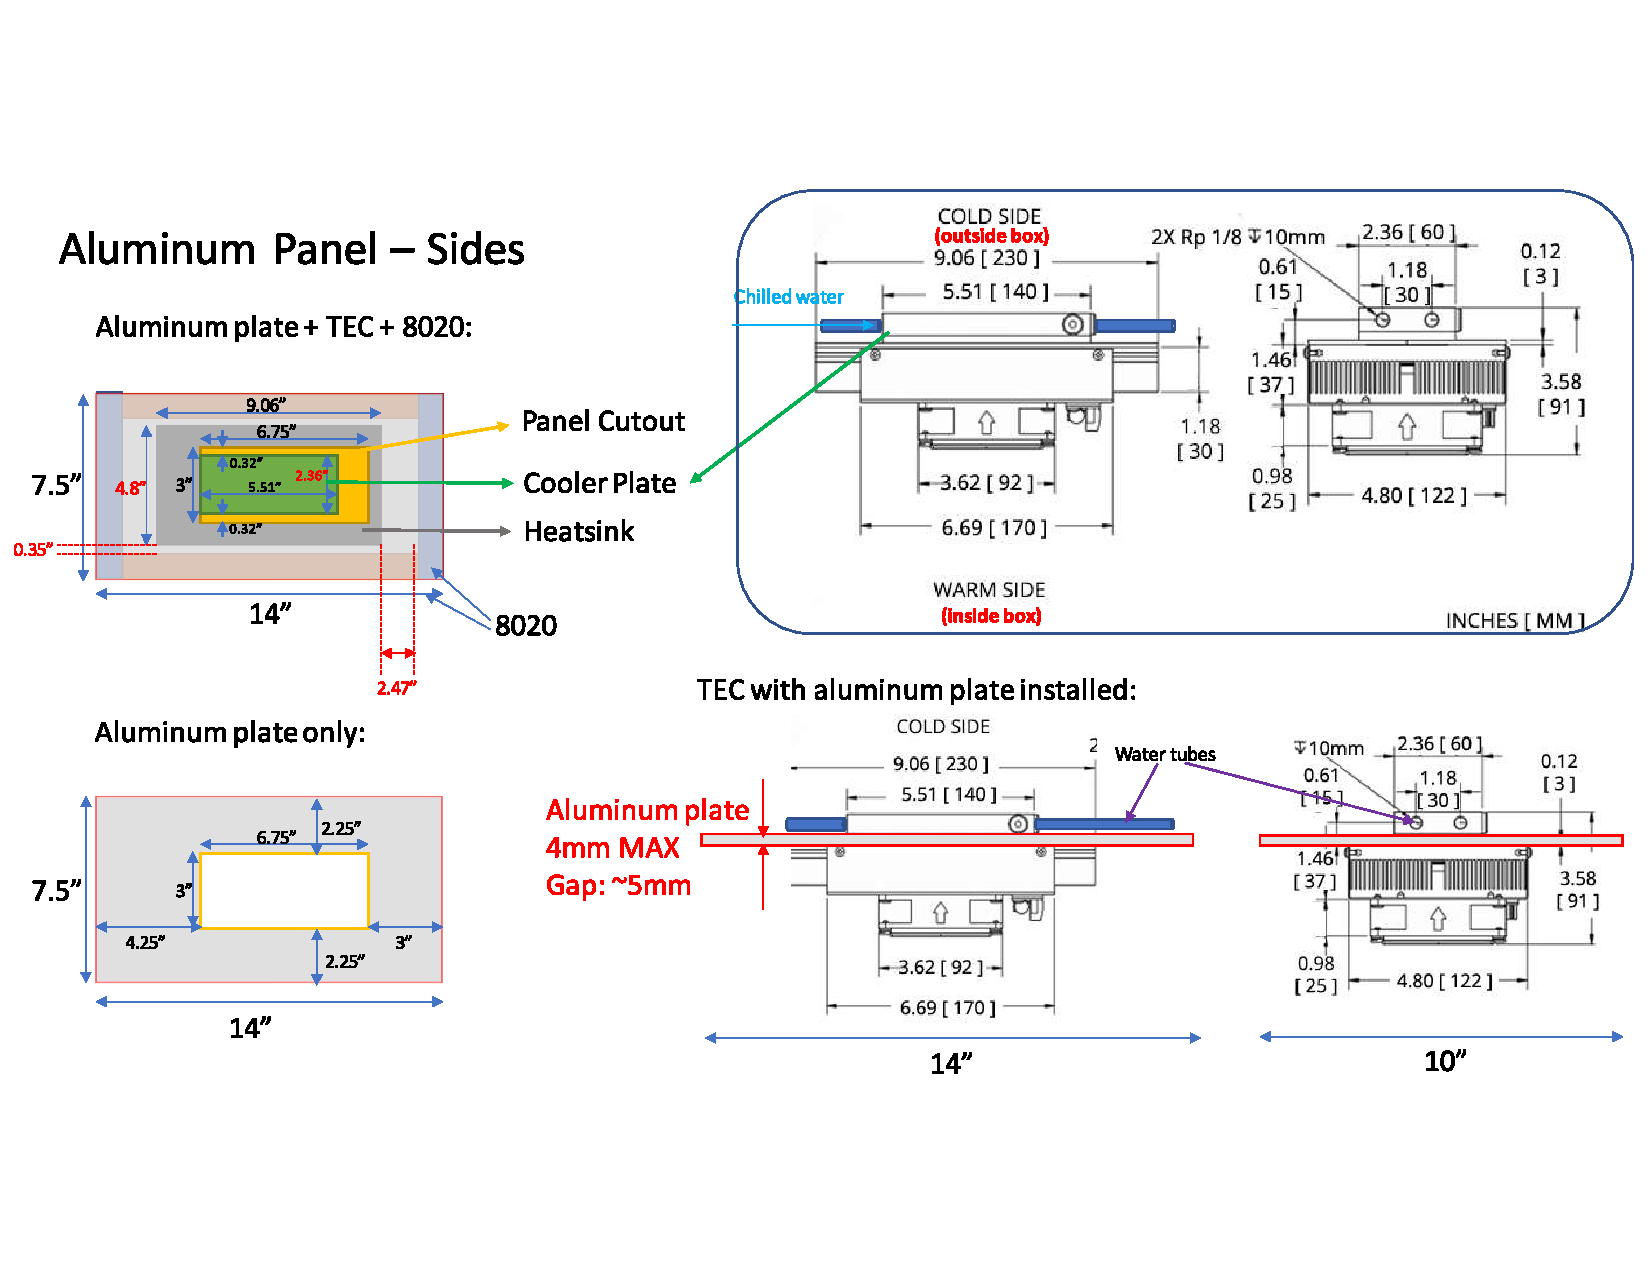
\includegraphics[width=1\textwidth]{Images/network_box_TEC_mount_sides.pdf}
    \caption{Mounting plate for TECs on sides of box. Courtesy Arian Noori.}
    \label{fig:box_TEC_mount_side}
\end{sidewaysfigure}

\newpage

\begin{sidewaysfigure}[!ht]
    \centering
    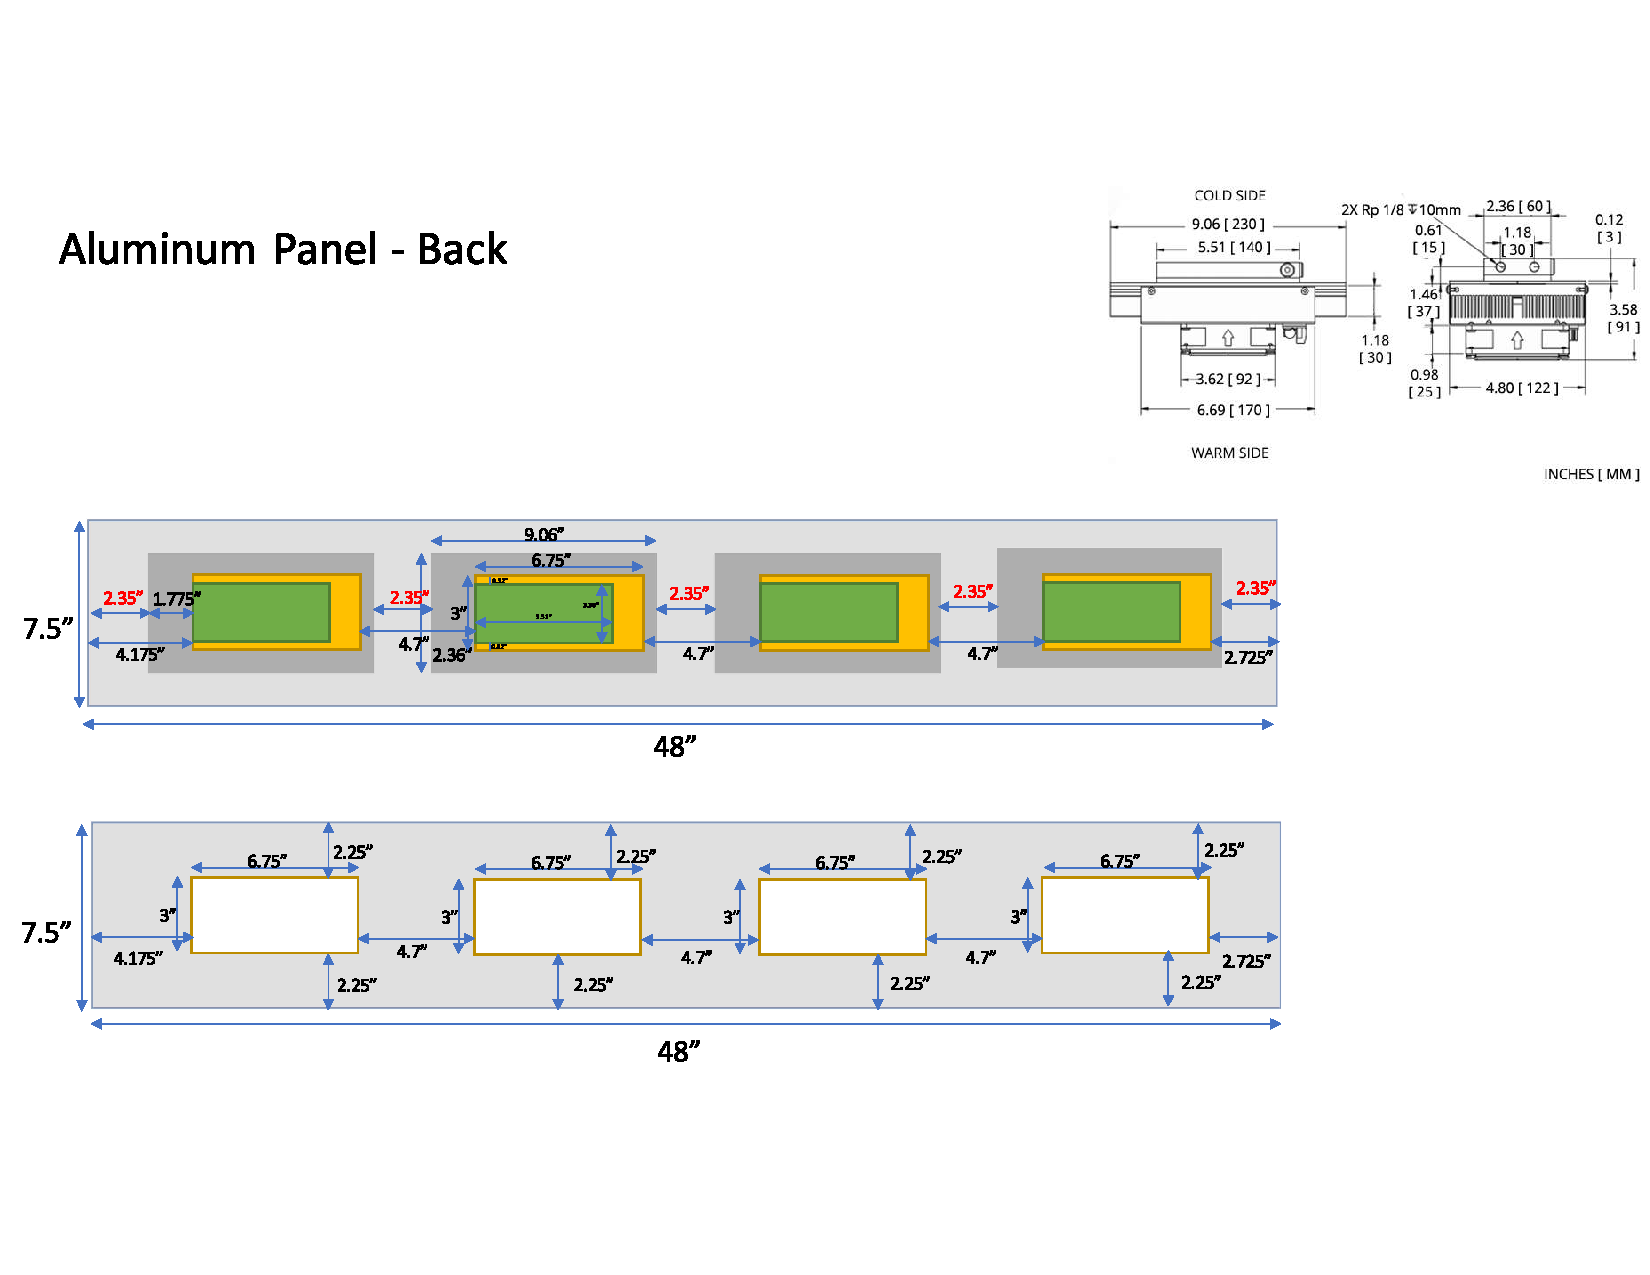
\includegraphics[width=1\textwidth]{Images/network_box_TEC_mount_back.pdf}
    \caption{Mounting plate for TECs on back of box. Courtesy Arian Noori.}
    \label{fig:box_TEC_mount_back}
\end{sidewaysfigure}

\newpage